\documentclass{article}
\usepackage{graphicx} % Required for inserting images
\usepackage{amsmath}
\usepackage[colorlinks=true, pdfstartview=FitV, linkcolor=blue, citecolor=blue, urlcolor=blue]{hyperref}
\usepackage{babel}
\usepackage{har2nat}
\usepackage{float}
\usepackage[top=1.1in, bottom=1.1in, left=1.15in, right=1.15in]{geometry}
\usepackage{booktabs}
\usepackage{amssymb}
\usepackage{dsfont}
\DeclareMathOperator*{\argmax}{arg\,max}
\DeclareMathOperator*{\argmin}{arg\,min}

\title{Lista 3 - Organização Industrial}
\author{Arthur M. Rodrigues}
\date{October 2023}


\begin{document}

\maketitle

Decisão dinâmica em $t$ do nível de estoque $I_t \in \{ 0, 1, 2, ...\}$, que possui custo $D(I_t) = \delta I_t^2$; $n_t \in \{0, 1, 2, ...\}$ é a quantidade demandada (exógeno), de modo que $n_t \leq I_t \implies R_t = pn_t$ e $n_t > I_t \implies R_t = pI_t$. Antes de observar $n_t$, firma decide encomendar $x_t \in \{0, 1, 2, ...\} = X$ (a ser entregue em $t+1$) com custo $cx_t + E$. Suponha $\beta = 0.95$.

\section*{Questão 1}

\subsection*{(a)}

Em $t$, as variáveis de estado são $I_t$ (endógena) e $n_t$ (exógena), enquanto a variável de controle é $x_t$ (e indiretamente $I_{t+1}$). A equação de Bellman é dada por:

\begin{equation}
    V(I) = \max_{x\in X} \{\mathbb{E}[ p\min(n,I) - cx - \mathds{1}_{(x>0)}E - \delta I^2] + \beta \mathbb{E}[V(I+x-\min(n,I)]\}
\end{equation}% E o subscrito de t na Bellman Equation?

Note que embora $n_t$ seja variável de estado, ela não é observada antes da escolha da firma. Portanto, a maximização de lucros da firma depende do valor esperado da demanda.

\subsection*{(b)}

O maior lucro possível para a firma em um dado período é $\Pi_t = pI_t - \delta I_t^2$, caso ela venda seu estoque completo e opte por não encomendar nenhuma unidade. Portanto, para que o lucro seja positivo, precisamos que:

\begin{equation*}
    pI_t - \delta I_t^2 \geq 0 \iff I_t(p - \delta I_t) \geq 0
\end{equation*}

Isto é, $\Pi_t \geq 0 \implies I_t \leq \frac{p}{\delta}$. Como $I_t$ é endógeno e resultado da escolha em $t-1$ (e $t$ e $t-1$ são arbitrários), temos que o estoque escolhido para a maximização de lucro é sempre finito (já que $p$ e $\delta$ são parâmetros finitos). Intuitivamente, a convexidade do custo de estocagem limita o valor do lucro possível mesmo para uma demanda arbitrariamente alta.

\subsection*{(c)}

Assumindo um choque que não seja magninitude suficientemente alta para que a firma saia do mercado, esperamos que os parâmetros $(\delta, p, c, E)$ alterem a função política da firma da seguinte forma:\\[4pt]

$p$: Com o aumento do preço, a receita para um dada quantidade vendida aumenta. Assim, a quantidade que a firma deixaria de vender pela demanda ser maior do que o estoque se torna mais "valiosa", aumentando o custo de subestimar a demanda. Espera-se que a firma então esteja disposta a carregar um estoque maior e, tudo mais constante, aumente a quantidade encomendada para os níveis de estoque em que realiza encomendas se torne mais propensa a realizar uma encomenda para dado nível de estoque.\\[4pt]

$\delta$: Com o aumento do custo de estoque, cada unidade não vendida torna-se mais custosa para a firma. Ou seja, aumenta-se o custo de superestimar a demanda. Espera-se que a firma deseje um estoque menor e, tudo mais constante, reduza a quantidade encomendada para os níveis de estoque em que realiza encomendas e se torne menos propensa a realizar uma encomenda para dado nível de estoque.\\[4pt]

$E$: Com o aumento no custo fixo de realizar uma encomenda, encomendas pequenas ficaram relativamente mais caras (tudo mais constante). Assim, esperamos que a firma encomende menos vezes (ou seja, apenas para quantidades menores de estoque) e que realize encomendas maiores quando opta por realizá-las. \\[4pt]

$c$: Para uma redução no custo unitário da mercadoria encomendada, encomendas pequenas ficaram relativamente mais caras (se o custo fixo de encomenda $E$ se mantiver constante, efeito análogo a um aumento de $E$). Assim, também esperamos que a firma realize encomendas maiores quando opta por realizá-las.

\section*{Questão 2}

\subsection*{(a)}\label{2a}

A partir dos dados de estoque e fluxo de encomendas, conseguimos inferir o número de vendas $n^*_t = I_{t+1} - (I_t + x_t)$ para os períodos $t = 1$ até $t = 29$. Ao gerar um histograma\footnote{Para esta e todas as  outras análises realizadas na Questão 2, retiramos as firmas $id = 1$ e $id = 9$, pois apresentam 0 em todas as variáveis para todas as observações.}, verificamos que a quantidade vendida varia entre 1 e 8 unidades com frequência similar.

\begin{figure}[H]
    \centering
    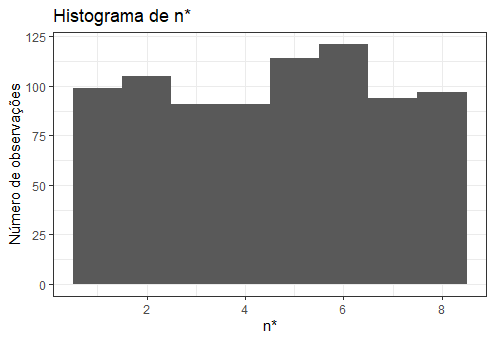
\includegraphics[width=0.5\linewidth]{figs and tabs/hist_nstar.png}
    \caption{Distribuição observada de $n^*_t$}
    \label{fig:histn}
\end{figure}

Entretanto, ao analisar a relação entre cada observação de $I_t$ e $n^*_t$, percebemos que 257 das 812 observações possuem $n^*_t > I_t$ (contra 114 com $n^*_t = I_t$ e 441 com $n^*_t = I_t$). Parece que a dinâmica proposta de encomendas não se aplica diretamente aos dados, e algumas encomendas realizadas chegaram antes da semana terminar, viabilizando que a empresa continuasse vendendo mesmo quando a demanda observada foi maior que o estoque inicial. Criamos uma variável de estoque expandido $I_{ex, t} = I_t + x_t$ para criar uma base restrita removendo observações com $n^*_t = I_t$ ou $n^*_t = I_{ex, t}$, visto que que a demanda nesses casos não está bem identificada (pois não sabemos se $n^*_t$ é a demanda real ou está subestimada pela restrição de estoque)\footnote{Note que o acontecimento de $n^*_t = I_t$ ou $n^*_t = I_{ex, t}$ não é exógeno, pois a probabilidade da firma possuir cada nível de estoque não é constante. Entretanto, a base restrita só possui 123 observações a menos que a base não restrita, de modo que a magnitude deste problema não deve ser alta.}. Regredimos $I_t$ em $n_t$ na base completa e restrita.

\begin{table}[H]
\begingroup
\centering
\begin{tabular}{lcc}
   \tabularnewline \midrule \midrule
   Dependent Variable: & \multicolumn{2}{c}{$n^*_t$}\\
   Model:         & (1)           & (2)\\  
   \midrule
   \emph{Variables}\\
   Constant       & 4.592$^{***}$ & 4.586$^{***}$\\   
                  & (0.1551)      & (0.1679)\\   
   $I_t$           & -0.0118       & -0.0365\\   
                  & (0.0242)      & (0.0255)\\   
   \midrule
   \emph{Fit statistics}\\
   Observations   & 812           & 689\\  
   R$^2$          & 0.00029       & 0.00299\\  
   Adjusted R$^2$ & -0.00094      & 0.00154\\  
   \midrule \midrule
   \multicolumn{3}{l}{\emph{IID standard-errors in parentheses}}\\
   \multicolumn{3}{l}{\emph{Signif. Codes: ***: 0.01, **: 0.05, *: 0.1}}\\
\end{tabular}
\par\endgroup
    \caption{Regressão do nível de estoque e quantidade vendida}
    \label{tab:regs}
\end{table}

Como nenhum dos coeficientes é significante, consideramos que o nível de estoque e a demanda são independentes, de modo que $\mathbb{E}[n_t | I_t] = \mathbb{E}[n_t]$. Outra preocupação é se há correlação serial na demanda (i.e., se $n_{t-1}$ afeta $\mathbb{E}[n_t]$). Para verificar se esse é o caso, regredimos a quantidade vendida na quantidade vendida no período seguinte:%Estimamos a matriz de transição observada entre $n^*_t$ e $n^*_{t+1}$ e 

\begin{table}[H]
\begingroup
\centering
\begin{tabular}{lc}
   \tabularnewline \midrule \midrule
   Dependent Variable: & $n^*_{t+1}$\\   
   Model:              & (1)\\  
   \midrule
   \emph{Variables}\\
   Constant            & 4.565$^{***}$\\   
                       & (0.1899)\\   
   $n^*_t$                & -0.0178\\   
                       & (0.0383)\\   
   \midrule
   \emph{Fit statistics}\\
   Observations        & 670\\  
   R$^2$               & 0.00032\\  
   Adjusted R$^2$      & -0.00117\\  
   \midrule \midrule
   \multicolumn{2}{l}{\emph{IID standard-errors in parentheses}}\\
   \multicolumn{2}{l}{\emph{Signif. Codes: ***: 0.01, **: 0.05, *: 0.1}}\\
\end{tabular}
\par\endgroup
    \caption{Regressão da quantidade vendida hoje e no período seguinte}
    \label{tab:my_label}
\end{table}

Mais uma vez, não encontramos coeficientes significativos, e portanto consideramos que $\mathbb{E}[n_t | n_{t-1}] = \mathbb{E}[n_t]$. Para estimar a distribuição da demanda que utilizaremos nas questões seguintes, vamos testar a hipótese de que a probabilidade de ocorrência de um nível de demanda é igual para todos os valores entre 1 e 8. Para isto, vamos utilizar o Teste qui-quadrado de Pearson para avaliar a qualidade do ajuste em relação aos dados observados para uma distribuição uniforme discreta com suporte entre 1 e 8.

\begin{table}[H]
    \centering
\begin{tabular}{l|r|r|r}
\hline
  & Test Statistic & Degrees of Freedom & P-Value\\
\hline
Chi squared & 0.4659061 & 7 & 0.999562\\
\hline
\end{tabular}
    \caption{Teste qui-quadrado de Pearson - base completa}
    \label{tab:my_label}
\end{table}

\begin{table}[H]
    \centering
\begin{tabular}{l|r|r|r}
\hline
  & Test Statistic & Degrees of Freedom & P-Value\\
\hline
Chi squared & 0.6136328 & 7 & 0.998915\\
\hline
\end{tabular}
    \caption{Teste qui-quadrado de Pearson - base restrita}
    \label{tab:gof2}
\end{table}


Rejeitamos a hipótese nula de que a distribuição observada é diferente da proposta na base completa e restrita. Assim, vamos considerar $n_t \sim \mathcal{U}\{1,8\}$ iid para os exercícios subsequentes\footnote{Dada a forma da função lucro, precisamos calcular $\mathbb{E}[n | n \leq I]$. Se $n_t \sim \mathcal{U}\{1,8\}$ então $\mathbb{E}[n | n \leq I] = 0$ se $I=0$, $\mathbb{E}[n | n \leq I] = (I+1)/2$ se $I \in \{1,..., 8\}$ e $\mathbb{E}[n | n \leq I] = 9/2$ se $I \in \{9, ..., 13\}$}.

\subsection*{(b)}% fazer disclaimer sobre o n_t enquanto variavel de estado

Queremos estimar a probabilidade de escolha de cada nível de encomendas para um determinado estoque $P_t (x | I)$.\footnote{Mais precisamente, $P_t (x | I, \mathbb{E}[n_t])$. Como assumimos $n_t$ iid, vamos omitir $n_t$ da notação de todas as funções que dependem do vetor de estados.} Para tal, vamos utilizar um método não paramétrico a partir da distribuição de encomendas observadas nos dados. A primeira etapa é calcular a probabilidade conjunta observada para os níveis de encomendas e estoque:

\begin{figure}[H]
    \centering
    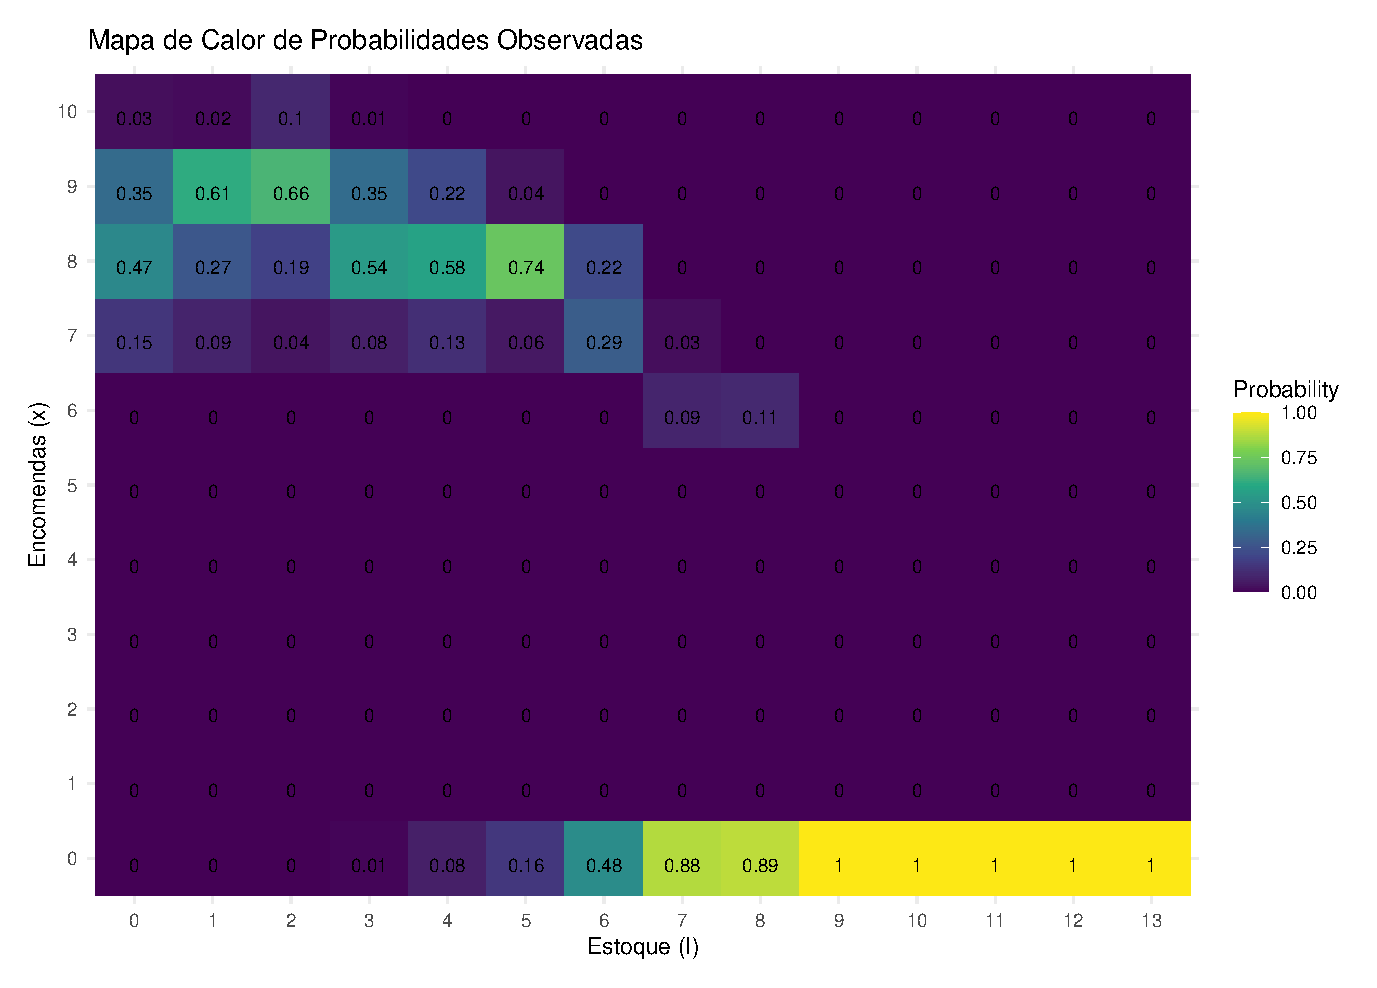
\includegraphics[width=\textwidth]{figs and tabs/prob_mat_xt_it.eps}
    \caption{Probabilidades Observadas de Pares Estoque x Encomendas}
    \label{fig:enter-label}
\end{figure}

Podemos visualizar que há relação clara entre escolha de $x_t$ e a realização de $I_t$: para níveis de estoque baixos, a firma opta por por realizar encomendas (usualmente entre 7 e 9 unidades), e à medida que o estoque do período aumenta, menor a probabilidade de realizar encomendas (a partir de $I_t = 9$ não observamos mais encomendas nos dados). Entretanto, o modelo teórico da Questão 1 não se verifica literalmente. Isso, pois o modelo proposto é determinístico, e se $\mathbb{E}[n_t$] é iid a firma sempre optará pela mesma encomenda para dado nível de estoque. Portanto, para estimar a função política vamos supor que o payoff da firma é aditivamente separável entre o lucro esperado e um vetor de choques específico para cada escolha $\nu_t = (\nu_t(1), \nu_t(2), ..., \nu_t(X))$. A firma escolhe a ação $x$ que satisfaz:

\begin{equation*}
    v(x,I)+\nu(x)\geq v(x',I)+\nu(x')\quad\forall x'\in X
\end{equation*}

Assumindo $\nu \sim Gumbel$, podemos realizar a inversão de Hotz-Miller e obter:

\begin{equation}\label{hotzmiller}
    v(x^{\prime},I)-v_i(x,I)=\ln(P'(x^{\prime}|I))-\ln(P'(x|I))
\end{equation}

Essa igualdade nos permite calcular a função valor normalizada $\tilde{v}(x,I)$ para cada escolha (normalizando $\tilde{v}(0,I) = 0 \quad \forall I$ e comparando com cada $x^{\prime}$ possível). Para isso, realizamos uma suavização de Laplace para calcular probabilidade modificada $P'(x | I)$, de modo a remover os remover os eventos com probabilidade zero e impedir valores arbitrariamente negativos resultantes dos logaritmos da Equação (\ref{hotzmiller}). A suavização é dada por:

\begin{equation*}
    P'(x_i | I_j) = \frac{(count(x_i, y_j) + \alpha)}{(\sum_{k} (count(x_k, y_j) + \alpha))}
\end{equation*}

E definimos $\alpha = 0.1$. Assim, calculamos o valor $\tilde{v}(x,I)$ de cada escolha possível em cada nível de estoque, dada a suavização da amostra observada. Os resultados podem ser visualizados na Figura \ref{fig:valuefunction}:

\begin{figure}[H]
    \centering
    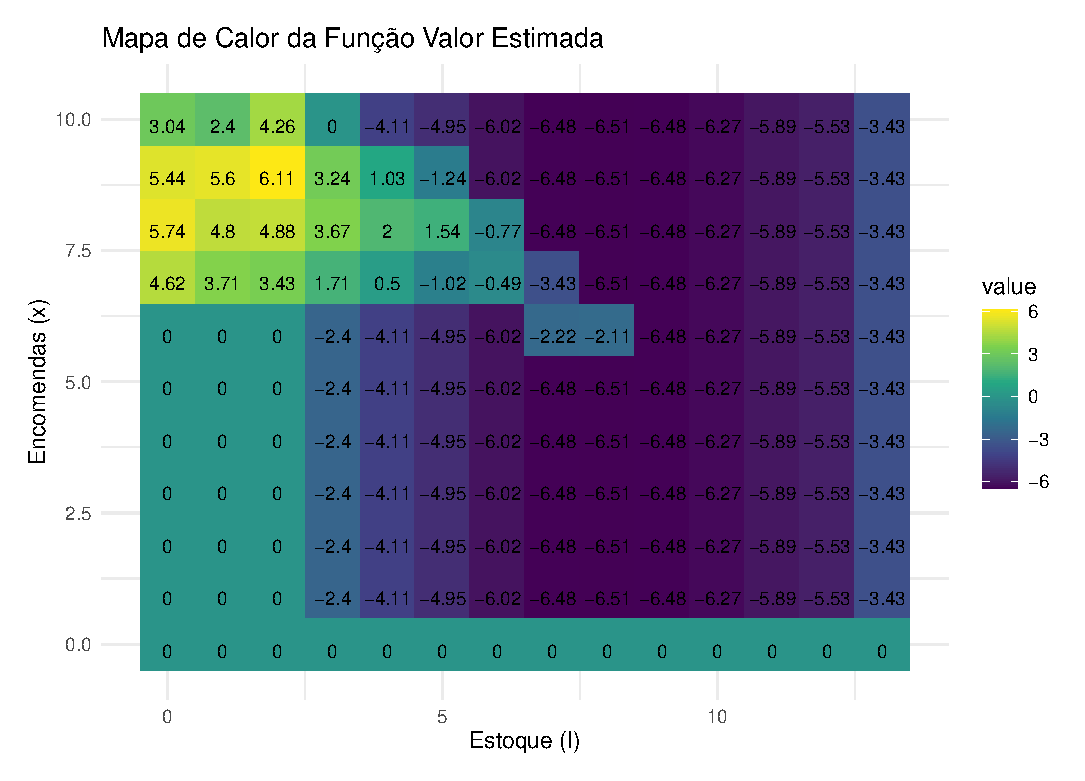
\includegraphics{figs and tabs/value_function.eps}
    \caption{Valor de cada Encomenda para cada Estoque Estimado}
    \label{fig:valuefunction}
\end{figure}

Replicamos várias vezes a última coluna da matriz para poder especificar escolhas das firmas para níveis de estoque até $I = 100$ (assumindo valores equivalentes à escolha em $I=13$). Então, a função política estimada a partir dos dados assume a forma:

\begin{equation*}
    x(I,\nu) = \argmax_x \{ \tilde{v}(x, I) + \nu_x \}
\end{equation*}

Para o restante da lista, utilizaremos a notação $x$ para definir a ação ($a$ na notação do BBL) e $x(I,\nu)$ para definir a função política ($\sigma$ na notação do BBL).

\section*{Questão 3}

\subsection*{(a)}

No modelo teórico proposto na Questão 1, o valor esperado do fluxo dos lucros descontados é dado por:

\begin{equation*}
    \begin{aligned}
    V(I,x(I,\nu))=\mathbb{E}\bigg[\sum_{t=0}^\infty\beta^t \left(p\min(n_t,I_t) - cx(I_t,\nu_t) - \mathds{1}_{(x_t>0)}E - \delta I_t^2 + \nu_t\right)  \bigg|I_0=I; p,c,E,\delta,\bigg]
    \end{aligned}
\end{equation*}

Pela linearidade da função lucro nos parâmetros, podemos definir $\theta = (p,c,E,\delta)$ e escrever:

\begin{equation*}
    V(I,x(I,\nu);\theta)= \mathbb{E}\bigg[\sum_{t=0}^\infty\beta^t \left(  \min(n_t,I_t), -x(I_t, \nu_t), \mathds{1}_{(x_t>0)}, I_t^2 \right) \bigg] \cdot \theta = \mathbb{E}\bigg[\sum_{t=0}^\infty\beta^t \Psi(x(I_t, \nu_t), I_t) \bigg] \cdot \theta
\end{equation*}

Então, definimos $W(I,x(I,\nu)) = \mathbb{E}\bigg[\sum_{t=0}^\infty\beta^t \Psi(x(I_t, \nu_t), I_t) \bigg]$. Essa simplificação é útil pois os componentes de $W$ não dependem dos parâmetros, de modo que a a simulação de $W$ pode ser realizada de forma independente antes da estimação de $\theta$, o que reduz bastante o requisito computacional do exercício. Para simular um dado $W(I)$, realizamos as seguintes etapas:

\begin{enumerate}
    \item Definimos $I_0 = I$ e sorteamos um choque $\nu_0$
    \item Definimos a ação da firma x($I,\nu_0$) e calculamos $\beta^0 \Psi(x(I, \nu_0), I)$
    \item Sorteamos $n_t$ e calculamos $I_{t+1} = I_t + x(I_t,\nu_t) - n_t$
    \item Repetimos o passos 1-3 por $T$ períodos e obtemos $W(\cdot) = \sum_{t=0}^T\beta^t \Psi(x(I_t, \nu_t), I_t)$
\end{enumerate}

Para melhorar a simulação, tomamos a média dos resultados para cada nível de estoque inicial de $N$ paths simulados.

\subsection*{(b)}

Vamos calcular os $W$s explicitados na seção anterior com $T = 100$ períodos e $N = 100$ paths. O código que realiza essa estimação em R está disponível no anexo \textit{'Lista3ArthurRodrigues.R'}. Considerando os níveis de estoque inicial de 0 a 11 (níveis com mais de 25 observações nos dados), essa simulação nos retorna uma matriz com 12 linhas (uma referente a cada estoque inicial cogitado $I_0$) e quatro colunas (pois $\Psi(\cdot)$ é um vetor de quatro elementos).


Para estimar os parâmetros a partir do modelo de BBL, também precisaremos especificar funções política alterativas cujos resultados serão comparados com os da política inferida a partir dos dados. Esses choques foram simulados a partir da função valor normalizada obtida na questão 2.b, de modo que $v'(x,I) = \tilde{v}(x,I) + \epsilon$, com $\epsilon \sim U[-2,2]$. Ao dar choques pequenos na matriz de valores, na prática fazemos com que, para dado $\nu$, a firma escolha níveis de encomenda marginalmente menos atrativos (por exemplo, escolher encomendar 7 ou 9 unidades ao invés de 8 quando $I=0$ ou optar por não encomendar nenhuma unidade quando $I=5$). Esse tipo de alteração no comportamento é justamente o que esperaríamos para uma mudança nos parâmetros $c$, $\delta$, $E$ ou $p$, como discutido no item 1.c. 


A partir disso, conseguimos especificar funções escolha alternativas $x'(I, \nu)$ e estimar $W' \def W(x'(I, \nu), I)$. Realizamos 10 choques $\epsilon \sim U[-2,2]$ que nos retornam 10 matrizes $W'$ distintas com dimensão 12x4.

Assim, as condições de equilíbrio são dadas por:

\begin{equation*}
    \theta \cdot W(x(I, \nu), I) \geq \theta \cdot W'(x'(I, \nu), I) \quad \quad \forall I, x'(I, \nu)
\end{equation*}



\subsection*{(c)}

A partir das $k \in \{1, 2, ..., 120\}$ condições de equilíbrio  calculadas no item (b), fixamos $\beta = 0.95$ e $p=10$, e encontramos o vetor $\hat{\theta}$ que satisfaz:

\begin{equation*}
    \widehat{\theta}:=\arg\min_{\theta}\sum_{k = 1}^K \theta \cdot [W - W']
\end{equation*}

Os resultados da estimação podem ser vistos na tabela abaixo:

\begin{table}[H]
    \centering
    \begin{tabular}{lr}
    Parâmetros & Estimativa \\
    \hline \hline
       $c$  & 1.73 \\
       $E$  &  19 \\
       $\delta$ & 0.12
    \end{tabular}
    \caption{Parâmetros Estimados}
    \label{tab:my_label}
\end{table}

Dado o preço de \$10 por unidade de mercadoria, o valor financeiro de uma encomenda de 8 unidades (o tamanho de encomenda mais comum nos dados) é de \$80. Os parâmetros estimados indicam que inicialmente essa encomenda custaria $8 \times 1.73 + 19 \approx \$32.8$. Para cada período que essas mercadorias não forem vendidas, há um custo adicional de $0.12 \times 8^2 \approx 7.7$.

\section*{Questão 4}

Para visualizar o impacto de uma mudança de preços dados os parâmetros estimados, realizaremos o processo de \textit{Value function iteration} (VFI) para o novo preço de $p=11$. Utilizaremos o modelo proposto na Questão 1, isto é, sem choques no lucro. Assim, o procedimento de VFI prevê o seguinte passo a passo:

\begin{enumerate}
    \item Defina um vetor $V[I]$, indexado pelos valores possíveis da variável de estado $I$ e atribua valores iniciais arbitrários (aqui, $V(I) = \left( 1, 1, ..., 1 \right)$).
    \item Atualize o vetor a partir da equação de Bellman e do $V$ proposto no passo 1: $V'[I] = \max_x \{ \pi(\theta,x,V) + \beta \sum_{n=1}^8 P(n) V[\Tilde{I}]$ \}, onde $\Tilde{I}$ é definido pela lei de movimento do estoque ($I_{t+1} = I_t + x_t - \min(n_t,I_t)$).
    \item Repita a atualização com $V = V'$ até a convergência de todos os elementos do vetor\footnote{Isto é, $\max(|V-V'|) < \epsilon$ para um $\epsilon$ suficientemente baixo}.
    \item Recupere a função política pra cada nível $I$ de estoque a partir equação de Bellman com o vetor $V[I]$ convergido.
\end{enumerate}

A partir desta receita, primeiro estimamos a função política ótima calculada com o preço original de $p=10$ e os parâmetros $\hat{\theta}$ estimados na questão anterior. A Tabela \ref{tab:VFI1} mostra os resultados deste procedimento e, para efeitos de comparação, a escolha com maior frequência de observações para cada nível de estoque na amostra.

\begin{table}[H]
    \centering
    \begin{tabular}{lcc}
    \hline
    Estoque ($I$) & \multicolumn{2}{c}{Encomenda ($x$)} \\
    & Moda Obs. & VFI com $\widehat{\theta}$ e $p=10$\\
    \hline \hline
       0  & 8 & 9 \\
       1  &  9 & 9 \\
       2 & 9 & 9 \\
       3 & 8 & 9  \\
       4 & 8 & 8  \\
       5 & 8 & 8  \\
       6 & 0 & 0  \\
       7 & 0 & 0 \\
       8 & 0 & 0 \\
       9 & 0 & 0 \\
       10 & 0 & 0 \\
       11 & 0 & 0 \\
       12 & 0 & 0 \\
       13 & 0 & 0 \\
    \end{tabular}
    \caption{Função Política com $p=10$}
    \label{tab:VFI1}
\end{table}

A função política obtida por VFI a partir de $\hat{\theta}$ estimado e $p=10$ é bem similar à escolha observada, o que indica que os parâmetros obtidos conseguem explicar bem o comportamento das firmas nos dados. Agora, vamos simular a função política no cenário contrafactual em que $p=11$. Os resultados encontrados a partir do mesmo processo de VFI com o novo nível de preço são:


\begin{table}[H]
    \centering
    \begin{tabular}{lc}
    \hline
       Estoque($I$)  & Encomenda ($x$) \\
       & VFI com $\hat{\theta}$ e $p=11$ \\
       \hline\hline
        0 & 10\\
        1 & 10\\
        2 & 9\\
        3 & 9\\
        4 & 9\\
        5 & 8\\
        6 & 8\\
        7 & 0\\
        8 & 0\\
        9 & 0\\
        10 & 0\\
        11 & 0\\
        12 & 0\\
        13 & 0\\
    \end{tabular}
    \caption{Função Política com $p=11$}
    \label{tab:my_label}
\end{table}

Como esperado, um aumento do nível de preços aumenta o tamanho das encomendas e a propensão da firma a realizá-las. Para o novo preço, a empresa encomendaria uma unidade a mais nos períodos com estoque igual a 0, 1 e 4 (em comparação com o VFI para $p=10$). Além disso, ela optaria por encomendar 8 unidades quando $I=6$, quando no nível de preços anterior sua decisão era por não realizar encomendas.

%\bibliographystyle{ecta}
%\bibliography{references}

\end{document}
